\documentclass[twoside,11pt]{article}
\usepackage[utf8]{inputenc}
\usepackage[T1]{fontenc}
\usepackage{lmodern}
\usepackage{amsmath, mathtools, bm}
\usepackage{booktabs}
\usepackage[preprint]{jmlr2e}
\usepackage{microtype}
\emergencystretch=3em

\newcommand{\Dl}{\bm{\Delta}}
\newcommand{\HH}{\bm{H}}
\newcommand{\TT}{\mathbb{T}^{2}}
\newcommand{\RR}{\mathbb{R}}
\newcommand{\PR}{\mathrm{PR}}

\title{What Does a Game-Trained Embedding Learn?\\
Strategy Ensembles versus Latent Overhead in Pursuit--Evasion}
\author{Raul Jimenez\textsuperscript{1,2}, Oleksii Ignatenko\textsuperscript{3}, Pavlos Protopapas\textsuperscript{4},\\
Leonid Sarieddine\textsuperscript{1,5}, Pau Sole-Vilaro\textsuperscript{1,5}, Pedro Tarancón-Álvarez\textsuperscript{1,5},\\
Pablo Tejerina\textsuperscript{1,5}, Nazar Tkach\textsuperscript{6}, Marisol Traforetti\textsuperscript{1,5}\\[1ex]
\normalfont\small\itshape
\textsuperscript{1}Institut de Ciències del Cosmos (ICC), Universitat de Barcelona, Barcelona, Spain\\
\textsuperscript{2}Institució Catalana de Recerca i Estudis Avançats (ICREA), Barcelona, Spain\\
\textsuperscript{3}Faculty of Applied Sciences, Ukrainian Catholic University, Lviv, Ukraine\\
\textsuperscript{4}Institute for Applied Computational Science, Harvard University, Cambridge, MA, USA\\
\textsuperscript{5}Departament de Física Quàntica i Astrofísica, Universitat de Barcelona, Barcelona, Spain\\
\textsuperscript{6}Department of Computer Science, National University of Kyiv-Mohyla Academy, Kyiv, Ukraine}
\date{July 2026}

\begin{document}

\jmlrheading{}{2026}{}{}{}{}{Jimenez et al.}
\ShortHeadings{What Does a Game-Trained Embedding Learn?}{Jimenez et al.}
\firstpageno{1}

\maketitle

\begin{abstract}
Multi-head physics-informed networks learn low-dimensional embeddings
of PDE solution families.  We train one such network on a two-player
pursuit--evasion game on the torus, a strategic rather than a
dynamical problem, and ask what its latent space encodes.  The key is
to separate two objects.  The \emph{strategy ensemble} --- the control
curves the heads output, one per initial condition --- is
low-dimensional, as saddle-point analysis predicts: its participation
ratio is $1.5$--$3.0$, close to the ideal value of $2$, and as
compressible as the Burgers family the architecture was designed for.
This rank is learned, not built in: game training collapses a planted
rank-$9$ ensemble to rank $2$--$3$.  The \emph{shared latent curve} carries a larger overhead
($\PR = 5.4 \pm 0.9$) that no head uses.  Three controls trace this
overhead to the input featurisation rather than the game: its spectrum
breaks at the input Fourier bandwidth, it is uncorrelated with the
game's winding classes across eight runs, and its variance is set
mostly by the random initialisation ($4.7\!:\!1$ over the task
instance).  The two dimensionalities stay separate in all $43$
training runs and across a sweep of the speed difference that carries
the game through its capturability transition.  The game's topology does appear --- but as clusters of the strategy
ensemble ($6\times$ separation between winding classes), not as latent
dimensions.  We are also careful about one tempting reading: the
apparent asymmetry between the two players' spectra is partly an
artifact of head gain, and what survives that is unstable under
symmetric training, so we do not attribute it to the game's
$\inf$--$\sup$ structure.  Every claim has a matching control, and an
independently trained Hamilton--Jacobi--Isaacs critic checks the actor
at the value level; its own failure modes are the subject of a
companion paper.
\end{abstract}

\begin{keywords}
  game-trained embeddings, representation learning, pursuit--evasion
  differential games, physics-informed neural networks, participation ratio,
  strategy ensembles, interpretability
\end{keywords}

\section{Introduction}
\label{sec:intro}

When a physics-informed network embeds a family of PDE solutions, its
latent dimensions usually have a clear meaning: they parameterise the
family.  \citet{JimenezEmbeddings2026} show this for the Burgers
equation with a multi-head network --- a shared body maps the base
coordinates to a latent curve, and per-instance linear heads pick out
solutions --- with $90\%$ of the family's variance in $3$ of $20$
latent components.  It is tempting to reuse the architecture on a
harder problem and read its spectrum the same way: train it on a
two-player game and call the spectrum the dimensionality of strategic
behaviour.

We try exactly that, and the tempting reading fails --- while a
sharper one holds up.  The problem is a pursuit--evasion game on the
flat torus \citep{Isaacs1965, basar1999dynamic}: a pursuer $20\%$
faster than the evader over a fixed horizon, both built as head banks
on shared bodies and trained by self-play on a differentiable
capture-time loss.  For this geometry, differential-game theory
already says what the optimal open-loop strategies are --- constant
headings along the shortest displacement geodesic
\citep{evans1984differential} --- so it predicts, before any training,
the dimension of what the network is meant to learn.  That prediction
is about the \emph{strategy ensemble}: the control curves the network
outputs, one per initial condition.  It says nothing about the latent
curve, which sits upstream of the heads and can carry anything.

The multi-head architecture is not new here.  We take it from prior
work.  What is new is what we turn it on: a strategy embedding learned
purely from a game, and a way to separate the embedding's strategic
content from its overhead.  Our method is to define those two objects,
then attribute every observable to game structure, architecture, or
training protocol with explicit controls.  There are four main
findings.

\textbf{Two dimensionalities separate} (Section~\ref{sec:twodims}).
The strategy ensemble has participation ratio $1.5$--$3.0$ across
every protocol variant we ran.  This matches the constant-heading
analysis, and the ensemble is as compressible as the Burgers
family ($90\%$ of variance in $4$ of $32$ ensemble components,
against $3$ of $20$).  A warm-start control shows the rank is actively
selected rather than an architecture default: game training destroys
a pre-fitted ensemble of rank $9.3$ within $8{,}000$ iterations.  The
latent curve keeps $\PR = 5.4 \pm 0.9$, an overhead that no head uses
(stacked-head effective rank $\approx 2.5$).  The separation is not a
population accident.  In each of the $43$ training runs and snapshots
we produced, the latent $\PR$ exceeds the strategy-ensemble $\PR$ by
at least $1.69$, for both players.

\textbf{The overhead is featurisation residue}
(Section~\ref{sec:featurisation}).  Three independent experiments
point the same way.  The latent power spectrum breaks exactly at the
input Fourier bandwidth, and under a $K$-sweep the break
tracks $K$ ($6 \to 6$, $12 \to 10$, $24 \to 22$, with $98\%$ of latent
power below $K$ in every arm).  The overhead is unrelated to the
game's homotopy content across eight runs spanning $3$--$13$ winding
classes, including a control that varies sector count at matched
capturability.  And its variance splits $4.7\!:\!1$ into
parameter-initialisation and task-instance parts.  Training
\emph{reduces} latent $\PR$ from $\approx 10.4$ at initialisation.  The
game removes dimensions from the featurisation's default and stops
where optimisation pressure ends, not at a game-set scale.

\textbf{Topology appears as clusters, not dimensions}
(Section~\ref{sec:topology}).  Winding sectors are linearly cheap, for
a simple reason: saddle strategies are constant headings, and
constants span a $2$-plane in control space no matter how many sectors
they realise.  The data agree.  Within-class control families are
essentially rank-$1$ ($\PR\ 1.10$--$1.22$), and classes separate by
$6\times$ in metric distance.  So the game's homotopy content is real
and prominent, carried by cluster geometry that no spectral statistic
sees.

\textbf{The one tempting spectral asymmetry does not survive its
ablation} (Section~\ref{sec:asymmetry}).  Raw head spectra suggest a
pursuer--evader asymmetry.  A gauge lemma shows that raw head spectra
are not observables of the learned strategies at all, and the apparent
concentration \emph{inverts} under gauge fixing.  What survives is a
$2\times$ pursuer excess of intermediate-band temporal power, stable
across seeds.  This is exactly the kind of signature one would happily
attribute to the $\inf$--$\sup$ structure, and a second-variation
analysis even predicts its direction.  We set in advance the condition
that would rule that attribution out, ran the fully symmetrised
protocol at four seeds, and report the result: the excess becomes
seed-dependent ($\times 1.25$--$1.99$, straddling the pre-registered
threshold, with sign inversions in one seed).  We withhold the
attribution.  This negative result is one of the paper's more useful
ones: gauge invariance plus seed stability, the usual bar for ``real
effect'', was not enough.

Everything is trained under an \emph{honesty contract}: no analytic
value, no optimal controls, nothing in any loss that a solver could
not observe.  There is one exception, disclosed and measured
(Section~\ref{sec:setup}).  On the torus, the standard
distance-shaping regulariser is provably an affine image of the
analytic value, and it supplies almost all of the evader's learning
signal.  We prove the identity, measure the gradient shares, and show
with a from-scratch sweep that the ensemble-rank conclusions do not
depend on it.  An independently trained Hamilton--Jacobi--Isaacs
critic checks the actor at the value level (Section~\ref{sec:critic}).
The critic's own convergence and failure analysis, including why its
residual level cannot be read as quality, is a companion paper
\citep{companion2026critics}.  A note on terminology.  The \emph{actor}
is the whole self-play object, the coupled pursuer and evader
head-banks; we name a single player when we mean one.  The
\emph{critic} is the separately trained value network.  This is not
actor--critic in the reinforcement-learning sense: the critic never
feeds gradients to the actor, and the two are trained independently.
Proofs, the full audit trail, and all training artifacts are in the
supplementary repository.

\section{Game, prediction, architecture}
\label{sec:setup}

\paragraph{The game.}  Pursuer $P$ and evader $E$ move at speeds
$v_P = 1.2$, $v_E = 1$ on $\TT = [0, 2)^{2}$.  Capture means
$d_{\mathbb{T}}(x_E, x_P) \le \varepsilon = 0.08$ within horizon
$t_{\max} = 4$, where $d_{\mathbb{T}}$ is the min-image distance.  $P$
minimises a capture-time functional and $E$ maximises it.  In relative
displacement coordinates $\Dl = x_E - x_P$ the feedback game has
value $V^{*}(\Dl) =
(d_{\mathbb{T}}(\Dl) - \varepsilon)_{+}/(v_P - v_E)$, attained by
colinear play along the minimal displacement geodesic.  This is the
positional saddle of the Krasovskii--Subbotin theory
\citep{krasovskii_subbotin1988}.  Within reach
$(v_P - v_E)\,t_{\max} + \varepsilon = 0.88$, which is $59.7\%$ of the
state space, capture is forced.  Outside it the evader escapes the
horizon, so on the full state space the value is the horizon-capped
$V^{*} = \min\bigl(t_{\max},\,(d_{\mathbb{T}}(\Dl) - \varepsilon)_{+}/(v_P - v_E)\bigr)$
of the companion critic \citep{companion2026critics}, with the cap
inactive on the reachable set the actor is scored on.  We chose these
constants as representative, not tuned.  The value scale is
$1/(v_P - v_E)$, and the dimensionless reach ratio
$\rho = R/(L/2)$, with reach radius $R = (v_P - v_E)\,t_{\max} +
\varepsilon$ (here $\rho = 0.88$), places the forced-capture
region inside the domain but below the threshold $\rho = 1$ at which
capturable play reaches the antipodal ridge, the cut locus of $V^{*}$.
The one singular limit is $v_P \to v_E$, where the value diverges
and the capturable set collapses onto the capture disk.
Section~\ref{sec:params} sweeps $v_P - v_E$ across that transition and
finds the embedding dimensionalities unmoved by it.  Two facts matter
downstream.  First, the saddle
\emph{open-loop} controls are constant headings
$\hat u^{*}(t) \equiv \widehat{\Dl}_0$: the optimal strategy
manifold, as a subset of $L^{2}([0, t_{\max}]; \RR^{2})$, is the
image of a circle whose linear span is two-dimensional.  A faithful
embedding of optimal strategies should therefore have rank
$\approx 2$ plus soft-game corrections, \emph{regardless of the
game's homotopy content} (Proposition~\ref{prop:span}).  Second, the
open-loop game itself has no value: a committed evader concedes at
most $1.11$ (wrap-around interception caps the reachable-set
advantage), while open-loop play against an informed maximiser
concedes at least $1.66$.  So self-play converges, if anywhere,
to a protocol-selected equilibrium, and we treat the trained object
as exactly that.

\paragraph{Architecture and training.}  Following
\citet{JimenezEmbeddings2026}, each player is a bank of $N_h = 16$
linear heads over a shared body.  A $\tanh$ MLP maps Fourier features
of time ($K = 12$ harmonics) to a latent curve
$\HH_\alpha(t) \in \RR^{16}$, and head $j$, one per evader initial
condition, outputs the unit heading
$\hat u^{j}_\alpha(t) = W^{j}_\alpha \HH_\alpha(t) /
\|W^{j}_\alpha \HH_\alpha(t)\|$.  Trajectories are rolled out with a
differentiable integrator.  This gives a soft expected capture time
$\widehat{T}$ (a differentiable surrogate for the first-capture time,
averaged over rollout) and a terminal survival probability $\bar S$
per head.  The players optimise
\begin{equation}
\mathcal{L}_P
 = \widehat{T} + \lambda_{\rm nc}\,\bar S\, t_{\max}
 + \lambda_d \langle d_{\mathbb{T}}(\Dl) \rangle,
\qquad
\mathcal{L}_E
 = -\widehat{T} - \lambda_d \langle d_{\mathbb{T}}(\Dl) \rangle,
\label{eq:losses}
\end{equation}
where $\langle\cdot\rangle$ averages over the $16$ heads and rollout
time, $\lambda_{\rm nc}$ weights a no-capture penalty and $\lambda_d$
the distance shaping.  The shaping term uses the min-image distance
$d_{\mathbb{T}}$, the quantity that enters $V^{*}$, not the raw
Euclidean $\|\Dl\|$ (the code wraps to the nearest image).  Since
$\widehat{T}$ is a time and $d_{\mathbb{T}}$ a length, $\lambda_d = 5$
is a dimensional coupling, not a dimensionless relative weight.  The
survival bonus ($\lambda_{\rm nc} = 2$) is \emph{one-sided}, so the
game as optimised is not exactly zero-sum.  This is one of three
protocol asymmetries, with the $3\!:\!1$ pursuer:evader step ratio and
the $10\times$ learning-rate ratio (Adam at $10^{-2}/10^{-3}$), that
Section~\ref{sec:asymmetry} returns to.  Training runs $14{,}000$
alternating iterations after a pursuer-only warm-up.  All analytic
gradients are verified against central finite differences to relative
error $\le 7\times10^{-9}$.  No analytic value or control enters any
loss.  We drop the head-orthogonality penalty of
\citet{JimenezEmbeddings2026}.  There it fixes the latent gauge for a
stable PCA.  Here the strategy target is a known rank-two object
(Proposition~\ref{prop:span}), the gauge is removed post hoc by
Lemma~\ref{lem:gauge}, and the self-play equilibrium is
non-stationary, so a basis-fixing penalty on a moving target would
constrain the wrong thing.

\paragraph{The disclosed exception.}  On $\TT$, off the capture set,
$d_{\mathbb{T}}(\Dl) = (v_P - v_E)\,V^{*}(\Dl) + \varepsilon$
identically.  So the shaping gradient \emph{is} the value gradient up
to a positive constant, and shaping is value-shaping on this geometry.
(It is not on bounded geometries, where boundary play decouples
distance from value.)  Measured at the trained equilibrium, shaping
supplies $\approx\!100\%$ of the evader's parameter-gradient norm and
$6.4\%$ of the pursuer's, and annealing $\lambda_d \to 0$ mid-training
collapses the evader's gradient by a factor $\approx 45$.  The honest
statement of the training signal is therefore: the pursuer is trained
by the game, the evader largely by shaping.  Every ensemble-rank claim
below is checked against this dependence (Table~\ref{tab:controls},
C5).

\begin{table}[t]
\centering\footnotesize
\begin{tabular}{p{0.5cm}p{2.8cm}p{4.9cm}p{5.1cm}}
\toprule
 & control & design & outcome \\
\midrule
C7 & warm-start collapse & pre-fit a rank-$9.3$ curved heading family
(MSE $10^{-5}$), then switch on the game loss &
$\PR(Z_E)\,6.5 \to 2.5$, $\PR(Z_P)\,8.0 \to 1.6$ within $8$k
iterations: near-constancy is \emph{selected}, not a default \\[2pt]
C5 & shaping sweep & $\lambda_d \in \{0, 1, 5\}$ from scratch
(unshaped initialisation gradients $8.3/3.5$: trainable) &
$\PR(Z) = 1.6$--$3.0$ in all arms; rank robust; evader rank mildly
shaping-dependent ($2.98 \to 1.94$) \\[2pt]
C3 & bandwidth sweep & input harmonics $K \in \{6, 12, 24\}$, all
else fixed & spectral break at $k = 6, 10, 22$: tracks $K$;
$98\%$ of latent power below $K$ in every arm \\[2pt]
C4 & sector restriction, capturability-matched & baseline radius
multiset rotated into a $\pm 15^{\circ}$ diagonal sector; $4/16$
capturable split preserved exactly & winding classes $12 \to 4$;
$\PR(\HH_E) = 5.22$, indistinguishable from the seed mean: no
topology effect on the latent \\[2pt]
C1 & decoupled dispersion & $8$ init seeds at fixed ICs; $5$ IC
resamples at fixed init & $\PR(\HH_E) = 5.4 \pm 0.9$ vs
$5.94 \pm 0.41$: init variance dominates $4.7\times$ \\[2pt]
C2 & symmetrised training & exact zero-sum loss
(machine-checked), no warm-up, $1\!:\!1$ steps, equal learning
rates; $4$ seeds $\times$ $5$--$6$ snapshots & band-gap run means
$\times 1.25$--$1.99$, snapshot range $[0.66, 3.29]$:
seed-dependent; $\inf$--$\sup$ attribution withheld \\
\bottomrule
\end{tabular}
\caption{The attribution controls.  For each we fixed a two-sided
decision rule before running it, and outcomes are stated against those
rules.  C7 and C5 protect the strategy-rank claims, C3, C4 and C1 the
featurisation attribution, C2 the asymmetry reading.}
\label{tab:controls}
\end{table}

\section{Two dimensionalities}
\label{sec:twodims}

\paragraph{Definitions.}  The \emph{strategy ensemble} of player
$\alpha$ is the indexed family
$\mathcal{S}_\alpha = \{\hat u^{j}_\alpha(\cdot)\}_{j=1}^{16}$, the
object the game theory constrains.  We measure its linear dimension by
the participation ratio
$\PR = (\sum_i \lambda_i)^{2} / \sum_i \lambda_i^{2}$ of the temporal
covariance spectrum of the pre-normalisation head outputs
$Z^{j} = W^{j}\HH(t)$, and of the unit-heading curves.  We report
both.  The $\PR$ over $16$ curves carries a bootstrap uncertainty of
about half a unit, so ranges rather than decimals carry the
conclusions.  The \emph{latent curve} $\HH(t)$ is upstream, and the
rank chain
$\mathrm{rank}(Z) \le \min(\mathrm{rank}\,W_{\rm stack},\,
\mathrm{rank}_t\,\HH)$
makes $\PR(\HH)$ only an upper bound on strategy content: latent
directions no head reads are invisible to play.

\paragraph{Result.}  Section~\ref{sec:setup} predicts
$\PR(Z) \approx 2$ plus soft-game corrections.  We measure
$\PR(Z_E) = 2.99$ and $\PR(Z_P) = 1.91$ at the baseline.  Across
everything we ran (eight init seeds, five IC sets, the sector
restrictions, the shaping sweep, the warm-start run, and twenty-one
symmetric-protocol snapshots) the population range is
$[1.46,\,2.99]$.  At the threshold used in the source construction,
$90\%$ of ensemble variance sits in $4$ of $32$ components ($Z_E$; $3$
of $32$ for $Z_P$), against Burgers' $3$ of $20$.  So \emph{the game's
strategy family is as compressible as the PDE solution family}, not
less.  The latent curve, by contrast, holds
$\PR(\HH_E) = 5.4 \pm 0.9$ ($n = 8$ seeds; range $[3.65, 6.75]$),
none of it read by the heads: the stacked, gauge-fixed head matrix
has effective rank $2.5$ (evader) and $1.9$ (pursuer).  The two
populations do not overlap.  The within-run form of the statement is
sharpest: in all $43$ checkpoints, for both players,
$\PR(\HH)/\PR(Z) \ge 1.69$.

\paragraph{Rank two under stronger play.}  The trained actor captures
only $23\%$ of the capturable set (Section~\ref{sec:critic}), so a
sceptic could read its $\PR(Z) \approx 2$ as a property of \emph{this}
weak equilibrium rather than of the saddle Proposition~\ref{prop:span}
describes.  It is not.  On the capturable heads, where the pursuit
strategy is actually determined, the unit-heading ensemble has
$\PR \approx 1.7$ for the analytic constant-heading saddle,
$\approx 2.1$ for the mediocre actor, and $\approx 2.4$--$2.7$ (three
seeds) for the oracle-trained pursuer of Section~\ref{sec:coadapt},
which captures the whole set.  Optimal, near-optimal and mediocre
pursuit are all rank two where it can be read.  The $\PR \approx 2$
signature is a property of constant-heading play across strengths, not
an accident of this equilibrium.  (Over all $16$ heads the oracle's
rank inflates to $\approx 7$, but only because its uncapturable heads
chase evaders they cannot reach, so their headings are undetermined;
this is an artifact of the free heads.  The four capturable heads are
the meaningful sample, small enough that these figures carry the same
half-unit uncertainty.)

\paragraph{Selected, not default.}  Two controls rule out the readings
a sceptic tries first.  The architecture is not rank-limited: it fits
an arbitrary curved unit-heading family of $\PR = 9.3$ to MSE
$10^{-5}$.  Started \emph{from} that state, game training destroys the
rank within $8{,}000$ iterations (Table~\ref{tab:controls}, C7) and
converges onto the standard equilibrium.  The shaped game objective
actively selects near-constant strategies.  And the selection is not
an artifact of the value-equivalent shaping term: trained from scratch
at $\lambda_d \in \{0, 1, 5\}$, the ensemble rank stays in
$[1.6, 3.0]$ in every arm (C5), including the unshaped game, which
trains despite having no value to converge to.  What does move with
$\lambda_d$, the evader's rank within that range, is reported as
shaping-conditioned wherever it appears.

\section{The latent overhead is featurisation residue}
\label{sec:featurisation}

If the $\approx 5$-dimensional latent overhead encoded game
structure, it should respond to game quantities and be stable to
architectural ones.  The opposite holds on both counts.

\begin{figure}[t]
\centering
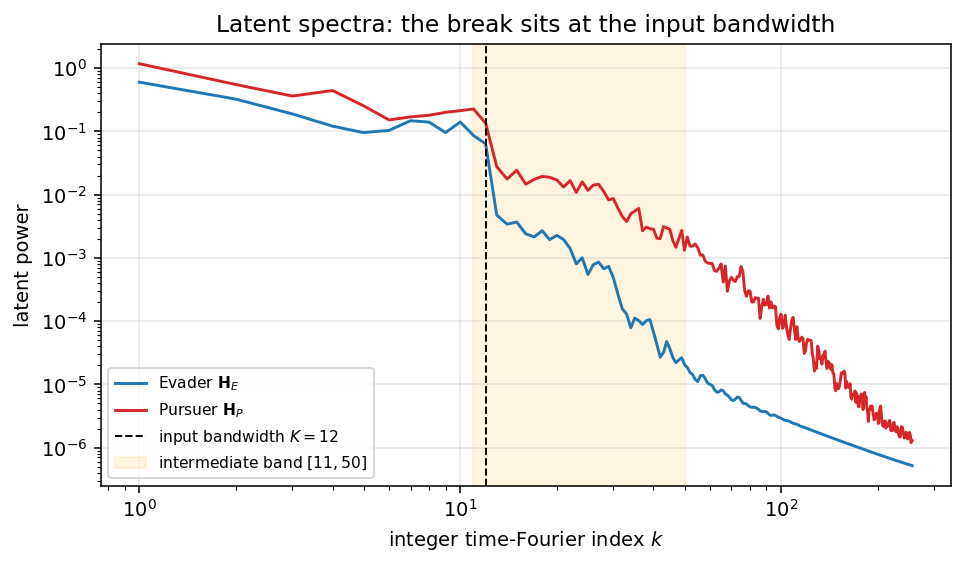
\includegraphics[width=0.72\textwidth]{fig_embed_intk_spectrum.png}
\caption{Integer-$k$ latent power spectra.  Both players' spectra are
flat through the passband and collapse just above the input bandwidth
$K = 12$ (dashed): between $k = 12$ and $k = 16$ the power drops by
$\approx 27\times$ (evader) and $\approx 9\times$ (pursuer).  Under the
bandwidth sweep the break follows $K$ ($6 \to 6$, $12 \to 10$, $24 \to 22$).
The shaded band $k \in [11, 50]$ is the intermediate band used for the
asymmetry statistics of Section~\ref{sec:asymmetry}.}
\label{fig:intk}
\end{figure}

\textbf{The spectral break is architectural.}  The latent power
spectrum (Figure~\ref{fig:intk}) breaks at the input bandwidth, and
the $K$-sweep (Table~\ref{tab:controls}, C3) moves the break with $K$,
not with any game scale.  A $\tanh$ body driven by band-limited
features populates frequencies above $K$ only through harmonics, and
that is what we see at every $K$.

\textbf{It is unrelated to game topology.}  We ran eight runs spanning
$3$--$13$ realised winding classes: five seeds, two sector
restrictions, and the capturability-matched diagonal-sector control
C4, which cuts the class count from $12$ to $4$ while preserving the
baseline's displacement-radius multiset and its $4/16$ capturable
split exactly.  Across them $\PR(\HH_E)$ shows no relation to class
count: the full-diversity minimum ($3.65$) undercuts the three-class
run ($5.02$), and C4 lands on the seed mean ($5.22$ against
$5.4 \pm 0.9$, $n = 8$).

\textbf{Its variance is a parameter-draw property.}  With initial
conditions fixed, eight init seeds give $\PR(\HH_E) = 5.4 \pm 0.9$.
With the init fixed, five IC resamples give $5.94 \pm 0.41$, a
$4.7\!:\!1$ ratio of variances (C1).  The ratio comes from small
samples ($n = 8$ and $n = 5$), so we read its direction (init
dominates IC) and its order of magnitude, not the precise figure.  And
training \emph{reduces} the latent rank from $\approx 10.4$ at
initialisation.  The overhead is what optimisation pressure has not yet
removed of the featurisation's default dimensionality, which is why it
sits at the bandwidth and varies with the seed.

\section{Topology: clusters, not dimensions}
\label{sec:topology}

\begin{proposition}[Constant curves are linearly cheap]
\label{prop:span}
Saddle open-loop controls on $\TT$ are constant headings; constant
$\RR^{2}$-valued curves span a two-dimensional subspace of
$L^{2}([0, t_{\max}]; \RR^{2})$.  Hence the linear dimension of the
ideal strategy manifold is $2$ independently of the number of
homotopy classes its members realise, and no participation ratio can
count winding sectors.
\end{proposition}

Linear statistics cannot see winding sectors.  Metric ones can.  We
label each head by the integer net winding of its evader trajectory,
the rounded net displacement over $[0, t_{\max}]$, per axis.  This
displacement is the lift to the universal cover (the evader velocity
integrated over the horizon, with no wrap applied), so $w$ is a
\emph{signed} class in $\pi_{1}(\mathbb{T}^{2}) = \mathbb{Z}^{2}$, not
a cyclic coordinate.  Unit headings bound it by the reach
$\|w\| \le v_E t_{\max}/L = 2$, and the extreme classes $w_x = \pm 2$
are opposite double-wraps, maximally separated in heading space
($L^{2} = 2$) rather than identified across a periodic seam.  The
baseline's $16$ trajectories realise $12$ classes, distributed
unevenly: one triple, two pairs, and nine singletons, so within-class
comparison rests on only five pairs.  Four of them are tight
($L^{2} \le 0.07$, a $\gtrsim 20\times$ separation from the cross-class
median $1.25$) and near rank-one ($\PR\ 1.1$--$1.2$).  One same-winding
pair is an outlier at $0.81$, which lifts the \emph{mean} within-class
distance to $0.20$ (a $6\times$ separation).  So the typical
within-class clustering is much tighter than the mean ratio suggests,
with one exception, on the minority of heads that have a same-class
neighbour at all.  Homotopy content is therefore prominent in the
ensemble, as \emph{cluster geometry} (Figure~\ref{fig:sectors}), where
it can be measured.  This resolves what would otherwise look like a
paradox in Section~\ref{sec:twodims}: a strategy family can be
topologically rich and two-dimensional at once, and this one is.

\begin{figure}[t]
\centering
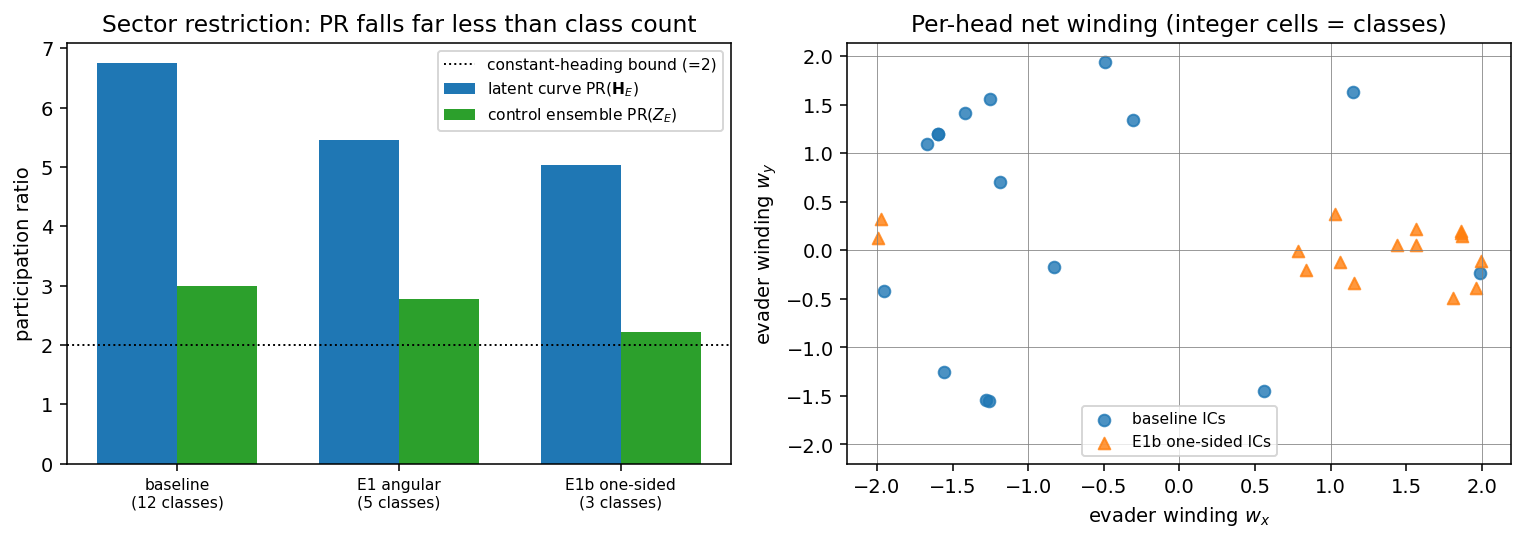
\includegraphics[width=\textwidth]{fig_embed_sectors.png}
\caption{Sector experiments.  Left: latent-curve $\PR$ (blue) vs
control-ensemble $\PR$ (green) across the baseline and two
sector-restricted runs; the dotted line is the constant-heading
bound of Proposition~\ref{prop:span}.  Right: per-head net winding
$w \in \RR^{2}$ for the baseline ($12$ integer classes, circles) and
the one-sided restriction ($3$ classes, triangles).  Restricting
sectors collapses the \emph{cluster count}; neither latent nor
ensemble rank follows it.}
\label{fig:sectors}
\end{figure}

\paragraph{Reflection control.}  The left--right structure of the
winding cloud is a property of the initial-condition distribution, not
of the winding coordinate.  We reflect the one-sided sector across the
$y$-axis ($x \to -x$) and retrain under an otherwise identical
protocol: same initialisation, optimiser, and $14{,}000$-iteration
budget.  This mirrors the cloud.  The $14/16$ heads that wound to
$w_x > 0$ under the $+x$ sector wind to $w_x < 0$ under the $-x$ sector
(mean $w_x$ moving from $+1.05$ to $-0.86$), and the two antipodal
wrap-arounds move from $w_x = -2$ to $w_x = +2$
(Figure~\ref{fig:reflection}).  Because a reflection carries the cloud
across $w_x = 0$, the winding is a genuine signed class in
$\mathbb{Z}^{2}$.  Were the axis cyclic, with $+2$ identified to $-2$,
the reflection would be a null operation.

\begin{figure}[t]
\centering
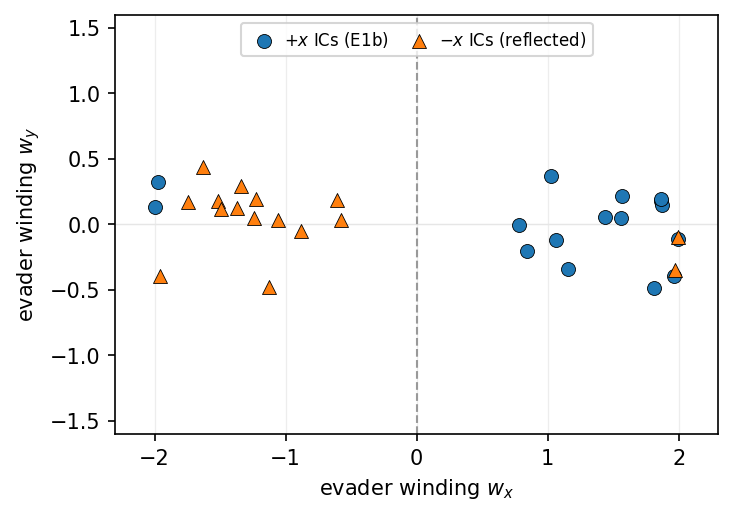
\includegraphics[width=0.6\textwidth]{fig_winding_reflection.png}
\caption{Reflection control.  Per-head evader winding for the one-sided
$+x$ sector (E1b, circles) and the same construction reflected to the
$-x$ sector and retrained identically (triangles).  The cloud mirrors
about $w_x = 0$ (dashed line): the asymmetry tracks the deliberately
one-sided initial conditions, and the signed winding does not wrap.}
\label{fig:reflection}
\end{figure}

\section{Parameter dependence}
\label{sec:params}

The constants of Section~\ref{sec:setup} are one point of a family, and
we ask whether the embedding picture survives as we move through it.
The controlling parameter is the speed difference
$\Delta v = v_P - v_E$.  It fixes the value scale $1/\Delta v$ and,
through the reach radius $R = \Delta v\,t_{\max} + \varepsilon$, the
reach ratio $\rho = R/(L/2)$.  On the flat torus the capturable share
of state space, $f(R)$, is the area fraction of $\{\Dl : d_{\mathbb{T}}
(\Dl) \le R\}$.  It is exactly computable and piecewise-smooth in the
parameters, with a curvature break at $\rho = 1$, where the
forced-capture disk first touches the antipodal cut locus, and
saturation at $R = L/\sqrt{2}$ (Figure~\ref{fig:params}a).  That break
is the one structural transition in the family: below it every
capturable trajectory is a short geodesic dash, above it capture wraps
around the torus and the antipodal ridge enters the capturable set.

We retrain the actor from scratch at eight speed differences
$\Delta v \in [0.05, 0.5]$, spanning $\rho \in [0.28, 2.08]$, three
initialisation seeds each, with the architecture, horizon, geometry and
evader IC set held fixed (the full $14{,}000$-iteration budget; the
$\Delta v = 0.2$ arm reproduces the qualitative split of
Section~\ref{sec:twodims}).  The result (Figure~\ref{fig:params}b) is
a clean negative: neither dimensionality tracks the structural break.
The strategy ensemble stays pinned near the constant-heading bound.
Its $\PR(Z_E) = 1.4$--$3.1$ across the whole family, marginally wider
than the fixed-$\Delta v$ runs' $1.5$--$3.0$ because the sweep reaches
into weaker- and stronger-game regimes, and it rises gently with
$\Delta v$ with no step at $\rho = 1$.  This shows
Proposition~\ref{prop:span} is not an artifact of the baseline
operating point: the strategies are two-dimensional wherever the game
is capturable at all.  The latent overhead stays at its featurisation
scale ($\PR(\HH_E) \approx 5$--$7$, no systematic trend in
$\Delta v$), exactly as Section~\ref{sec:featurisation} predicts for a
quantity set by the input bandwidth $K$ rather than by any game scale.
Capture performance, by contrast, rises with the capturable share as
it must (Figure~\ref{fig:params}a).  The game moves the actor's
behaviour across the transition, but not the dimension of its
representation.

\begin{figure}[t]
\centering
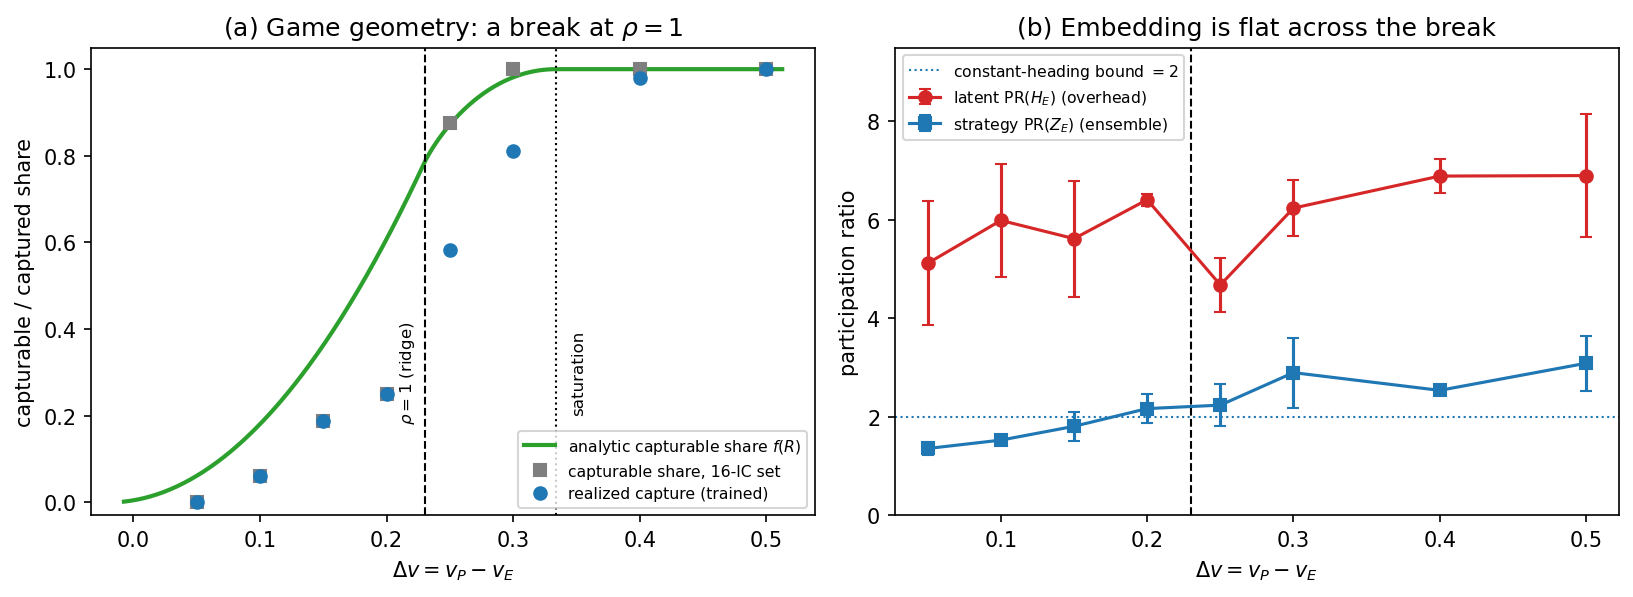
\includegraphics[width=\textwidth]{fig_dv_sweep.png}
\caption{Embedding structure across the speed-difference family.
(a)~The analytic capturable share $f(R)$ on $\TT$ is piecewise-smooth
with a curvature break at $\rho = 1$ (dashed) and saturation at
$R = L/\sqrt{2}$ (dotted); the fixed IC set's capturable share and the
trained actor's realised capture track it.  (b)~Latent
$\PR(\HH_E)$ and strategy-ensemble $\PR(Z_E)$ versus $\Delta v$
(mean\,$\pm$\,s.d., three seeds): the strategy rank stays at the
constant-heading bound and the latent rank at its featurisation scale
straight through the $\rho = 1$ break, so the representation does not
see the game's structural transition.}
\label{fig:params}
\end{figure}

\section{The asymmetry that was not attributable}
\label{sec:asymmetry}

The trained players differ, and the differences invite
game-theoretic readings.  We take apart the two we found most
tempting.

\begin{lemma}[Gauge freedom of the heads]
\label{lem:gauge}
The policy is invariant under per-head rescaling
$W^{j} \to c_j W^{j}$, $c_j > 0$: unit headings depend only on the
direction of $W^{j}\HH$.  Raw singular-value spectra of stacked head
matrices are therefore not observables of the learned strategies.
\end{lemma}

\begin{figure}[t]
\centering
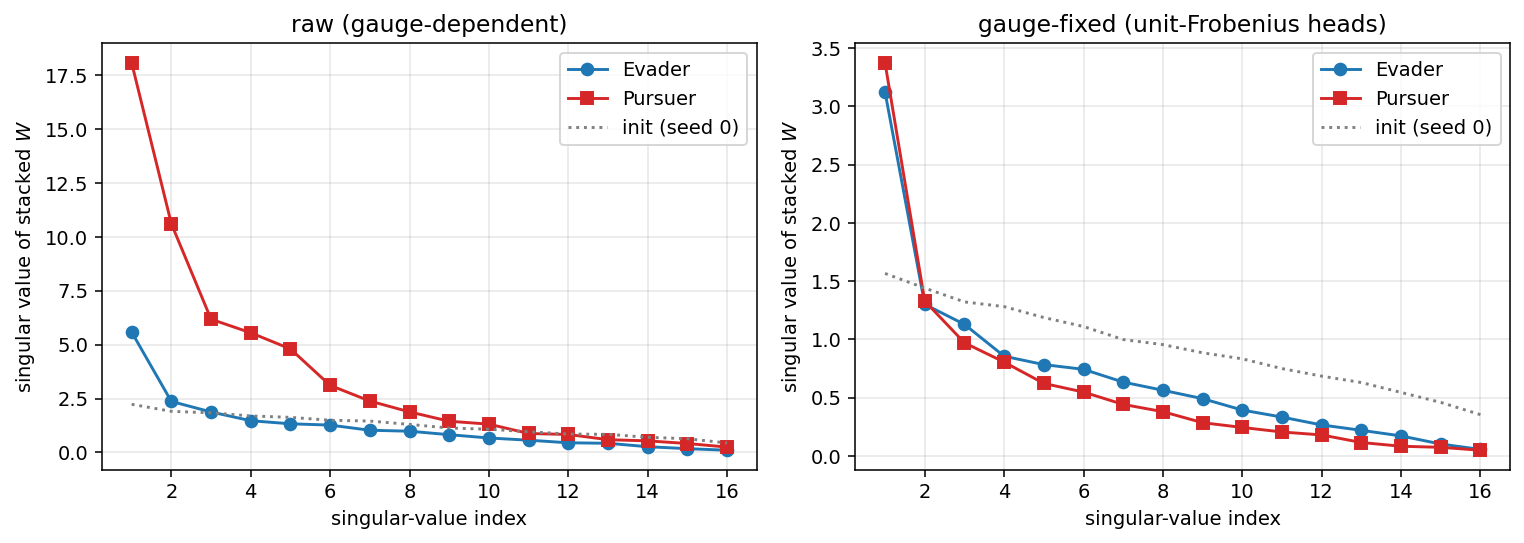
\includegraphics[width=\textwidth]{fig_embed_head_gauge.png}
\caption{Head singular values, raw vs gauge-fixed.  Left: raw
spectra, pursuer max $18.1$, evader max $5.6$.  Right: after fixing
each head to unit Frobenius norm the apparent concentration
\emph{inverts} (effective rank $2.53$ evader vs $1.91$ pursuer).  The
raw contrast tracks weight motion ($4.1\times$ vs $1.3\times$ the
initialisation norm), so it is optimisation gain, not strategy
structure.}
\label{fig:head_ortho}
\end{figure}

The raw head spectra differ by $3\times$ in scale between the players.
By Lemma~\ref{lem:gauge} this is gain, and gauge fixing inverts it
(Figure~\ref{fig:head_ortho}).  What survives gauge fixing is real: in
the unit-heading ensembles the intermediate band $k \in [11, 50]$
carries $30.3\%$ of the pursuer's temporal power against $15.8\%$ of
the evader's, a $\approx 2\times$ excess that persists when shaping is
annealed away ($22.7\%$ vs $11.5\%$) and is reproducible across seeds
under the baseline protocol ($\times 1.44$--$1.92$).  There is even
theory pointing the right way.  At the saddle, the second variation of
capture time weights pursuer heading perturbations by $v_P/v_E$ and
adds an $\varepsilon^{-1}$-concentrated endgame term that binds only on
capturing trajectories.  The minimising player keeps receiving
broadband curvature after the maximising player's objective has
saturated (soft no-capture mass $0.70$ at equilibrium).

But the trained asymmetry is confounded: the protocol itself treats
the players asymmetrically (one-sided survival bonus, $3\!:\!1$ steps,
$10\times$ learning-rate ratio).  We fixed a two-sided rule for the
deciding experiment: gap persists $\ge 1.5\times$ under a fully
symmetrised protocol $\Rightarrow$ attributable to the $\inf$--$\sup$
structure; collapse $\Rightarrow$ protocol artifact.  We then ran
exact zero-sum training (loss symmetry machine-checked each step, no
warm-up, $1\!:\!1$ steps, equal learning rates) at four seeds, five to
six snapshots each, the equilibrium being oscillatory as expected for
simultaneous gradient play \citep{mescheder2018gan,
daskalakis2018training}.  The outcome (Table~\ref{tab:controls}, C2):
run-mean gaps of $\times 1.25$, $1.51$, $1.64$, $1.99$, straddling the
threshold, with snapshot range $[0.66, 3.29]$ and sign inversions in
one seed, where the asymmetric protocol was seed-stable.  The rule
returns no verdict.  The raw-scale gap, meanwhile, equalises exactly
as the gauge analysis predicts ($\sigma_{\max}\ 12.5/12.5$).  We
therefore withhold the attribution: the asymmetry is at minimum
strongly protocol-shaped, and deciding whether any of it is
game-theoretic needs replication power this study does not have.  The
methodological point stands regardless.  A gauge-invariant,
seed-stable, theory-consistent signature was still protocol-sensitive,
and only a pre-registered ablation could say so.

\section{The equilibrium is protocol-limited, not capacity-limited}
\label{sec:coadapt}

The trained actor is a genuine but mediocre equilibrium (it captures a
minority of the capturable set, Section~\ref{sec:critic}), and
adversarial self-play is known to be unstable: simultaneous gradient
play in a zero-sum game rotates around the equilibrium rather than
converging to it \citep{mescheder2018gan, daskalakis2018training}, the
two-dimensional analogue of the limit cycles of rock--paper--scissors.
Is the mediocrity a limit of the open-loop \emph{networks} or of the
co-adaptive \emph{protocol}?  We separate the two by re-training the
pursuer under four protocols at matched budget, initial conditions,
architecture and seeds (three each), scoring the mean pursuit gap on
the analytically capturable heads and its late-training oscillation
(Figure~\ref{fig:protocols}).

Against a \emph{fixed} optimal evader, the constant-heading saddle of
Proposition~\ref{prop:span}, an oracle opponent that removes
co-adaptation entirely, the pursuer converges monotonically to full
capture (gap $1.4\times10^{-3}$, oscillation s.d.\ $5\times10^{-4}$).
A single open-loop head per initial condition has ample capacity to
realise optimal pursuit, so representation is not the bottleneck.  The
instability lives in the coupling.  Strict simultaneous ($1{:}1$) play
is oscillatory and seed-dependent (capture $0.75$--$1.0$, oscillation
up to $0.04$, one seed losing a head), the same signature the
symmetrised control of Section~\ref{sec:asymmetry} showed on the
spectral side.  Undamped alternating best response (train one player
toward convergence, switch, repeat) \emph{cycles}: pursuer and evader
alternately win outright (capture $0$ at the measured phase,
oscillation $0.17$, an order of magnitude above every other arm),
never settling.  This is exactly the best-response cycle that only
time-averaging (fictitious play) is known to close.  The baseline's
$3{:}1$ pursuer:evader step ratio is the steadiest of the co-adaptive
arms, its asymmetry damping the cycle.  The equilibrium's quality is
therefore a property of the training dynamics, not of the
representation.  That is the limit of the ``mediocre'' verdict, and the
reason the co-training plan of Section~\ref{sec:limits} must specify an
opponent schedule, not just a larger network.  (The oracle opponent
uses the analytic optimal strategy, so it is a diagnostic baseline,
outside the honesty contract, not a training method we advocate.  We
test only the pursuer this way.  The mirror arm, an evader against a
fixed optimal pursuer, is degenerate by construction, since a slower
evader has no escaping strategy against optimal faster pursuit, only
delay.)

\begin{figure}[t]
\centering
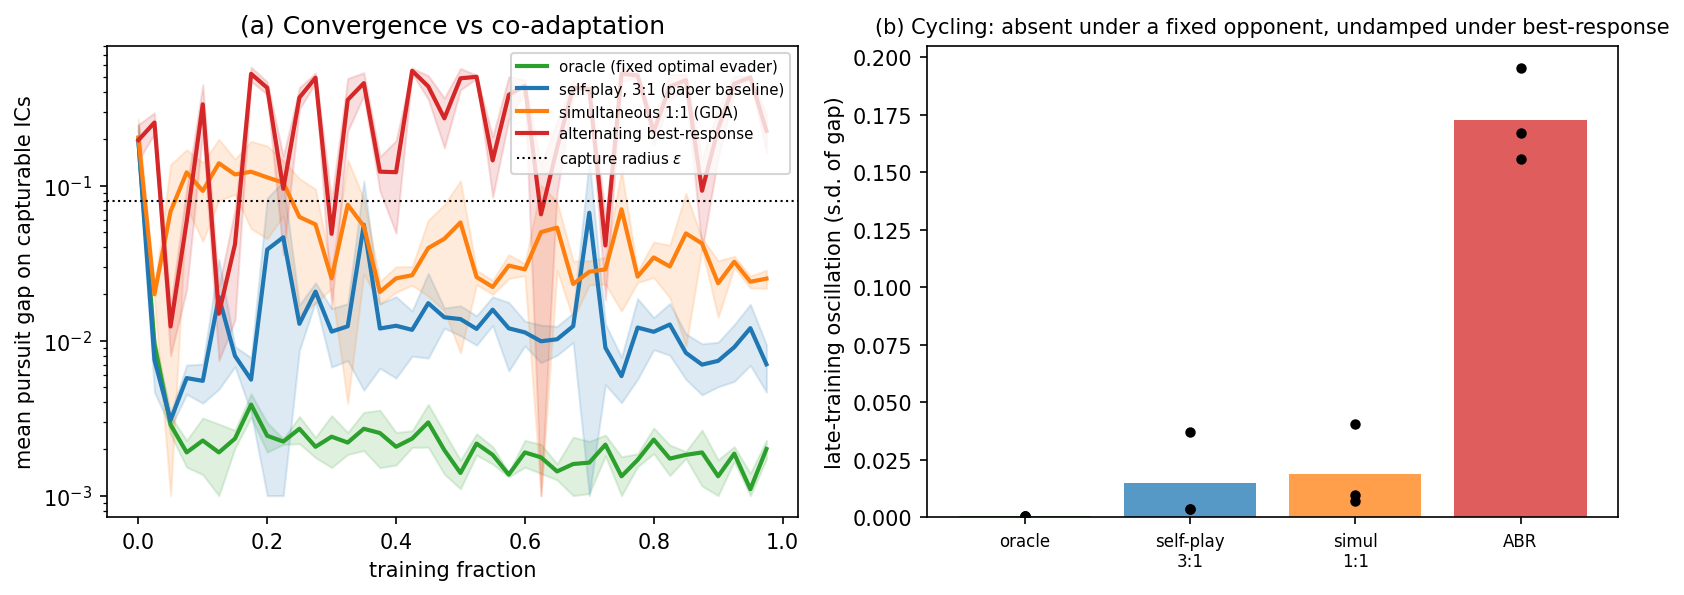
\includegraphics[width=\textwidth]{fig_protocols.png}
\caption{Actor training dynamics under four protocols (matched budget,
ICs, architecture; three seeds).  (a)~Mean pursuit gap on the
capturable heads vs training fraction (band: s.d.\ over seeds): the
oracle (fixed optimal evader) descends monotonically below the capture
radius; alternating best-response sawtooths between win and loss;
simultaneous $1{:}1$ oscillates; the $3{:}1$ baseline is damped.
(b)~Late-training oscillation amplitude grows monotonically with the
symmetry of the co-adaptation, from zero for the fixed opponent to
largest for alternating best-response.  Capacity is constant across
arms; only the coupling changes.}
\label{fig:protocols}
\end{figure}

\paragraph{Can an honest protocol recover the oracle's stability?}
The oracle removes co-adaptation by fixing the opponent to the analytic
optimum, which the honesty contract forbids.  We asked whether a
\emph{self-play} correction can recover its stability.  We tested the
standard game-optimisation fixes that provably tame cycling in
convex--concave games (extragradient, optimistic gradient
descent--ascent \citep{daskalakis2018training}, and iterate averaging)
on the identical $1{:}1$ setting, three seeds, at matched budget.  None
closes the gap (Figure~\ref{fig:honest}).  Ces\`aro
parameter-averaging is actively \emph{destructive} (capture collapses
to $0.4$): the iterates orbit a limit cycle rather than a point, and
their mean is a blurred, non-capturing policy.  Optimism and
extragradient are inconsistent across seeds (capture $0.58$--$0.83$,
oscillation still $10$--$100\times$ the oracle's).  We also tried the
combination the nonconvex min--max literature favours, optimistic GDA
with an exponential moving average of the iterate.  It attains the
\emph{lowest} oscillation of any honest arm, but only by trading
capture down to $0.58$, so it too stays out of the basin.  (Forcing the
smaller \emph{symmetric} step the convergence theory assumes makes it
worse: the pursuer needs its larger step to learn pursuit within
budget, and capture collapses.  The step asymmetry is load-bearing,
not merely a cycle-damper.)  Across the toolkit the honest methods
trace a capture--stability trade-off, and none enters the oracle basin
(Figure~\ref{fig:honest}a).  These methods are not wrong.  Their
guarantees are for convex--concave (or bilinear) games, while this
min--max problem is nonconvex--nonconcave, so the corrections do not
carry over directly.  Closing the honest-versus-oracle gap, a
self-play protocol that reaches the oracle basin without the oracle, is
a concrete open problem, and the quality--stability plane of
Figure~\ref{fig:honest}a is the yardstick we propose for it.

\begin{figure}[t]
\centering
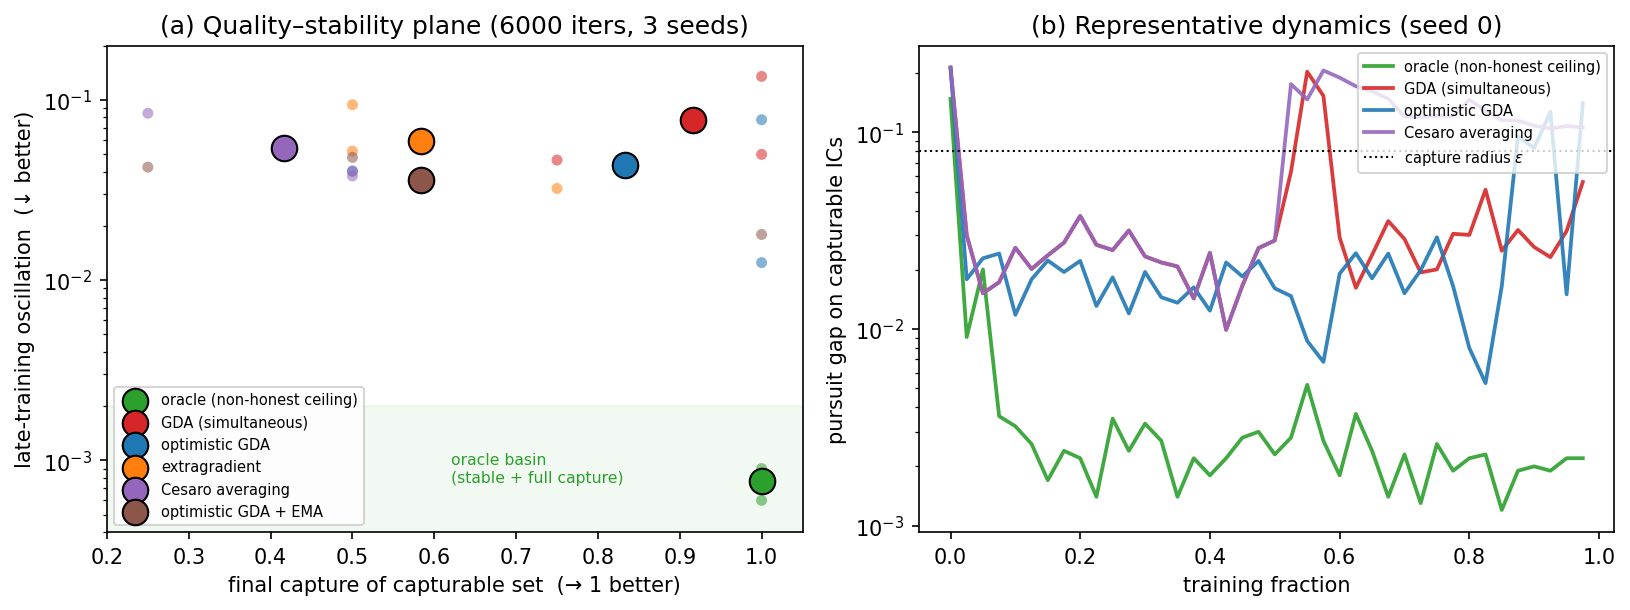
\includegraphics[width=\textwidth]{fig_honest.png}
\caption{Honest self-play corrections do not reach the oracle
(6{,}000 iterations, three seeds; consistent with a $12{,}000$-iteration
check).  (a)~Quality--stability plane: final capture (right is better)
versus late-training oscillation (down is better).  The oracle occupies
a stable, full-capture basin (shaded) that no honest correction enters
(simultaneous GDA, optimistic GDA, extragradient, Ces\`aro averaging,
or optimistic GDA with iterate EMA); large markers are protocol means,
small markers seeds.
(b)~Representative dynamics: the oracle converges and stays; GDA
oscillates; the averaged model sits high (its mean policy does not
capture).}
\label{fig:honest}
\end{figure}

\paragraph{Locating the gap with Shapley values.}  We cannot close the
gap, but we can say precisely where it lives.  Treating disjoint
frequency bands of the pursuer's time input as players, we compute the
exact Shapley attribution of capture (against the fixed optimal evader,
so both pursuers face the same task) for an oracle-trained and a
self-play-trained pursuer (Figure~\ref{fig:shap}).  The oracle builds
capture almost entirely from a \emph{low-frequency} heading
modulation: the $k \in [1,4]$ band carries $68\%$ of its capture, and
the linear, mid and high bands little.  The self-play pursuer never
acquires that band.  Every band's Shapley value is $\approx 0$, and
against the optimal evader it falls back on its constant-heading (DC)
response, capturing $0.17$ against the oracle's $1.00$ ($n = 3$ seeds).
The result has two parts.  As a diagnosis, the co-adaptation gap is a
\emph{specific missing component}, the low-frequency pursuit
correction, not a diffuse deficit.  Shapley localises it without
touching a weight, which is exactly its scope: an attribution of a
trained model, not a training method.  As independent corroboration of
Section~\ref{sec:twodims}, capture is carried by near-constant,
low-frequency headings, while the higher-frequency content (the latent
overhead) contributes essentially nothing to play, now confirmed by a
Shapley analysis rather than a spectral one.

\begin{figure}[t]
\centering
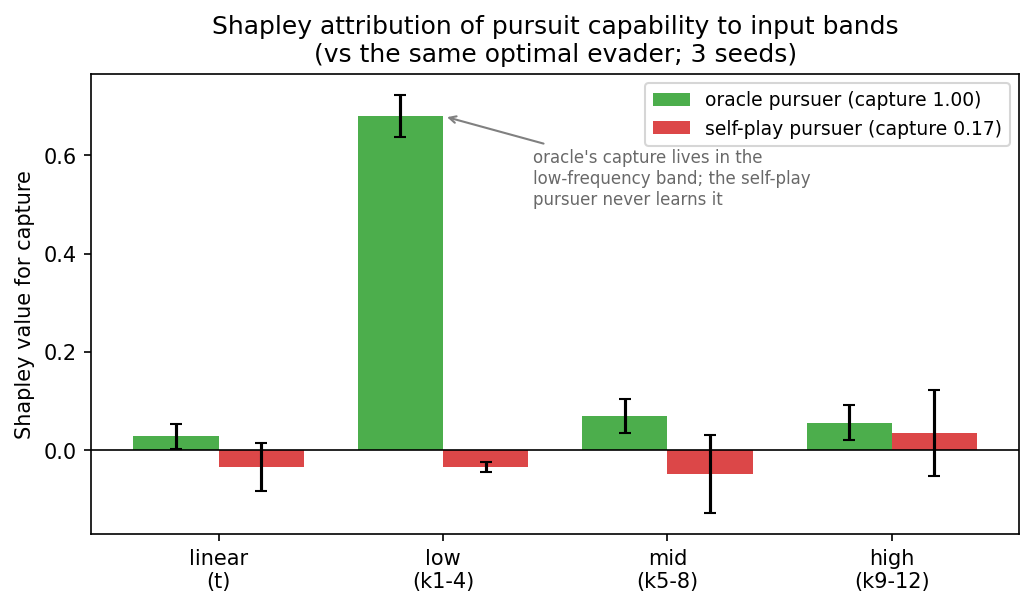
\includegraphics[width=0.74\textwidth]{fig_shap.png}
\caption{Exact grouped-Shapley attribution of capture to frequency
bands of the pursuer's time input, evaluated against the same optimal
evader (three seeds; masked features set to their time-mean).  The
oracle pursuer's capture concentrates in the low-frequency band; the
self-play pursuer acquires no useful band and reverts to its
constant-heading response.  Shapley locates the oracle gap (a missing
low-frequency modulation) but, computed on trained networks, does not
close it.}
\label{fig:shap}
\end{figure}

\section{Value-level verification}
\label{sec:critic}

A representation audit of a game-trained network needs an independent
standard of play.  We train a critic on the HJI residual of the
displacement-form game plus its two physical boundary conditions, again
nothing analytic, and use it three ways.  This verification critic runs
at the actor's horizon $t_{\max} = 4$ ($\rho = 0.88$), so the
capturability normalisation below is matched to the actor's reachable
set.  The companion paper's longer-horizon torus arm
($\tau_{\max} = 8$, $\rho = 1.7$) probes the ridge-active regime
separately.

\emph{Performance, normalised by capturability.}  The critic's
feedback policy captures $31\%$ of the analytically capturable test
set; the open-loop actor captures $23\%$.  (Unnormalised grid
fractions, $19\%$ and $14\%$, understate both, since only $59.7\%$
of the grid is capturable at all.)  The actor is a real equilibrium of
middling strength, which bounds the scope of every conclusion above.

\emph{The directional comparison factorises.}  Along rollouts, the
measured actor--critic alignment equals the product of each side's
alignment with the analytic saddle direction $\widehat{\Dl}$ to
within $0.03$ ($0.882 \times 0.484 = 0.427$ vs $0.433$ measured;
$0.882 \times 0.576 = 0.508$ vs $0.541$ with a stronger critic).  So
there is no actor--critic coupling beyond what the saddle direction
mediates, and the critic's gradient field is the bottleneck.  The
companion paper traces that bottleneck to the critic's parameterisation
rather than to residual training itself \citep{companion2026critics}.

\emph{Topology-level consistency is unpopulated at this
equilibrium.}  The companion paper's structured critic exposes a
homotopy selector validated exactly against the analytic pursuit
chart.  This enables a topology-level actor--critic consistency test:
do the actor's winding classes agree with the critic's active chart
along rollouts?  Run on this actor, the test returns a well-defined
empty verdict.  The only heads whose relative displacement ever
contests the antipodal ridge are the escaping, horizon-limited ones,
exactly where the selector is analytically degenerate, while every
capturable head stays clear of it.  Strategy topology and value
topology do not interact at the open-loop equilibrium.  This is one
more face of the actor's early commitment, and the concrete observable
that the co-training plan of Section~\ref{sec:limits} aims to
populate.

\emph{A null for the latent bridge.}  The natural conjecture that the
latent overhead encodes value information fails its control.  The
critic's value along rollouts is decoded from the top two latent
components at cross-validated $R^{2} = 0.46$, but from \emph{time
alone} at $0.53$.  The leading latent components are smooth functions
of $t$, so the decodability is not latent-specific.  We report this
null with the same standing as the positive results, and it closes the
last route back to ``the overhead is game content''.

\section{Related work}
\label{sec:related}

Neural approaches to pursuit--evasion and differential games mostly
\emph{solve} the game: multi-agent RL and self-play
\citep{lowe2017maddpg, baker2020emergent}, value-function and
reachability methods \citep{bansaltomlin2021deepreach}.  Our question
is different.  We ask what the trained representation contains, and we
are not aware of prior representation audits of game-trained
physics-informed architectures.  The construction and the latent-PCA
method are from \citet{JimenezEmbeddings2026}, and the Burgers
comparison is protocol-matched to that source (its variance thresholds
and standardisation conventions).  The training-signal disclosure
connects to the known sensitivity of self-play equilibria to
optimisation asymmetries \citep{mescheder2018gan,
daskalakis2018training}.  The critic builds on physics-informed
residual training \citep{Raissi2019, Karniadakis2021}.  Its failure
modes, and the standards under which any critic-derived number here
should be read, are developed in the companion paper
\citep{companion2026critics}.

\section{Limitations and outlook}
\label{sec:limits}

Ground truth here comes at a cost in scope.  All embedding conclusions
concern one game family on one geometry, at one equilibrium of an
open-loop actor that captures $23\%$ of the capturable set, and the
PDE-side comparison rests on a single source family.  Three extensions
would move the conclusions rather than tighten them.  A
\emph{closed-loop, state-conditioned actor} is the only one that could
alter the ensemble-rank story: feedback strategies are not constant
headings, so Proposition~\ref{prop:span} no longer bounds them.
\emph{Bounded geometries} (disk, ball, M\"obius strip) make the shaping
term harmless, since distance is provably not value-equivalent there,
which makes them the clean venue for repeating the embedding analysis.
And \emph{honest co-training} against the companion paper's structured
critic, whose validated homotopy selector meets this paper's winding
analysis at the topology level, is the planned route to a
value--representation bridge that our nulls show does not yet exist.  A
fourth extension is now open rather than closed.
Section~\ref{sec:params} varies the speed difference but holds
$\varepsilon$, $t_{\max}$ and $L$ fixed, and the clean piecewise
structure of the game geometry (Figure~\ref{fig:params}a) invites
promoting all four to \emph{conditioning inputs} of a single embedding.
That would map how the latent and strategy spectra deform across the
phase diagram.  From the piecewise-linearity of $V^{*}$ in these
parameters, we expect (and pre-register) smooth dependence broken only
at the capturability ($v_P \to v_E$) and ridge-activation
($\rho = 1$) transitions.  A fifth extension is more open-ended and
follows from Section~\ref{sec:coadapt}.  The honest--versus--oracle
stability gap left standing there motivates a \emph{purpose-built
nonconvex--nonconcave min--max optimiser}, an asymmetry-preserving
optimistic method with adaptive per-player preconditioning and
recency-weighted iterate averaging, aimed at reaching the oracle basin
under pure self-play.  The concrete first attempt we would make is
\emph{neural fictitious self-play} with an opponent pool (``league''
training), which averages the \emph{play} rather than the weights.
This is the version of averaging with zero-sum convergence guarantees,
and the one our parameter-averaging arm was a degenerate substitute
for.  It exposes the pursuer to strong, self-generated opponents
instead of only the current weak one.  This is a study in its own
right, so we pose it here, with the quality--stability plane
(Figure~\ref{fig:honest}a) as its benchmark, rather than attempt it.

The transferable method is smaller than the paper and easy to state:
define the embedded object before measuring it; predict its dimension
from theory; give every interpretive claim a pre-registered, two-sided
control; and let gauge lemmas and nulls kill readings early.  On this
game, that discipline turned a tempting headline (``strategic
behaviour is seven-dimensional'') into a sharper, better-supported
one.  The strategies are exactly as simple as the game theory says,
the extra dimensions belong to the featurisation, and the topology
lives in the metric, where the spectral statistics could not see it.

\section*{Reproducibility statement}
All training code (a from-scratch NumPy pipeline with every analytic
gradient verified against central finite differences to
$\le 7\times10^{-9}$), checkpoints for all $43$ runs and snapshots,
the analysis suite that regenerates every number and figure, and the
complete audit trail (pre-registered designs, decision rules, and the
per-control analysis records cited in Table~\ref{tab:controls}) are
versioned in the supplementary repository.  No result in this paper
depends on unreleased data or manual steps.

\section*{Acknowledgments}
P.T.-A.\ is supported by the project ``Dark Energy and the Origin of
the Universe'' (PRE2022-102220), funded by
MCIN/AEI/10.13039/501100011033.  Funding for the work of P.T.-A.,
P.T., L.S., P.S.-V., N.T., M.T.\ and R.J.\ was partially provided by
project PID2022-141125NB-I00 and the ``Center of Excellence María de
Maeztu 2020--2023'' award to the ICCUB (CEX2019-000918-M), funded by
MCIN/AEI/10.13039/501100011033.

\bibliographystyle{plainnat}
\begin{thebibliography}{20}

\bibitem[Baker et al.(2020)]{baker2020emergent}
B.~Baker, I.~Kanitscheider, T.~Markov, Y.~Wu, G.~Powell, B.~McGrew,
and I.~Mordatch.
\newblock Emergent tool use from multi-agent autocurricula.
\newblock In {\em International Conference on Learning
Representations}, 2020.

\bibitem[Bansal and Tomlin(2021)]{bansaltomlin2021deepreach}
S.~Bansal and C.~J.~Tomlin.
\newblock {DeepReach}: A deep learning approach to high-dimensional
reachability.
\newblock In {\em IEEE International Conference on Robotics and
Automation (ICRA)}, pages 1817--1824, 2021.

\bibitem[Ba\c{s}ar and Olsder(1999)]{basar1999dynamic}
T.~Ba\c{s}ar and G.~J.~Olsder.
\newblock {\em Dynamic Noncooperative Game Theory}.
\newblock SIAM Classics in Applied Mathematics, 2nd edition, 1999.

\bibitem[Companion paper(2026)]{companion2026critics}
Companion paper.
\newblock Low residual, wrong value: what sampled-residual training
cannot certify for {Hamilton--Jacobi--Isaacs} equations, and what fixes it.
\newblock 2026.  Submitted concurrently.

\bibitem[Daskalakis et al.(2018)]{daskalakis2018training}
C.~Daskalakis, A.~Ilyas, V.~Syrgkanis, and H.~Zeng.
\newblock Training {GANs} with optimism.
\newblock In {\em International Conference on Learning
Representations}, 2018.

\bibitem[Evans and Souganidis(1984)]{evans1984differential}
L.~C.~Evans and P.~E.~Souganidis.
\newblock Differential games and representation formulas for
solutions of {Hamilton--Jacobi--Isaacs} equations.
\newblock {\em Indiana University Mathematics Journal},
33(5):773--797, 1984.

\bibitem[Isaacs(1965)]{Isaacs1965}
R.~Isaacs.
\newblock {\em Differential Games}.
\newblock Wiley, New York, 1965.

\bibitem[Karniadakis et al.(2021)]{Karniadakis2021}
G.~E.~Karniadakis, I.~G.~Kevrekidis, L.~Lu, P.~Perdikaris, S.~Wang,
and L.~Yang.
\newblock Physics-informed machine learning.
\newblock {\em Nature Reviews Physics}, 3(6):422--440, 2021.

\bibitem[Krasovskii and Subbotin(1988)]{krasovskii_subbotin1988}
N.~N.~Krasovskii and A.~I.~Subbotin.
\newblock {\em Game-Theoretical Control Problems}.
\newblock Springer-Verlag, New York, 1988.
\newblock Translated from the Russian {\em Positional Differential
Games}, Nauka, Moscow, 1974.

\bibitem[Lowe et al.(2017)]{lowe2017maddpg}
R.~Lowe, Y.~Wu, A.~Tamar, J.~Harb, P.~Abbeel, and I.~Mordatch.
\newblock Multi-agent actor-critic for mixed cooperative-competitive
environments.
\newblock In {\em Advances in Neural Information Processing
Systems 30}, 2017.

\bibitem[Mescheder et al.(2018)]{mescheder2018gan}
L.~Mescheder, A.~Geiger, and S.~Nowozin.
\newblock Which training methods for {GANs} do actually converge?
\newblock In {\em International Conference on Machine Learning},
2018.

\bibitem[Raissi et al.(2019)]{Raissi2019}
M.~Raissi, P.~Perdikaris, and G.~E.~Karniadakis.
\newblock Physics-informed neural networks: A deep learning
framework for solving forward and inverse problems involving
nonlinear partial differential equations.
\newblock {\em Journal of Computational Physics}, 378:686--707,
2019.

\bibitem[Tarancón-Álvarez et al.(2026)]{JimenezEmbeddings2026}
P.~Tarancón-Álvarez, L.~Sarieddine, P.~Protopapas, and R.~Jimenez.
\newblock Learning embeddings of non-linear {PDEs}: the {Burgers'}
equation.
\newblock {\em arXiv:2603.07812}, 2026.

\end{thebibliography}

\end{document}
